%!TEX root = ../thesis.tex
%*******************************************************************************
%****************************** Sixth Chapter **********************************
%*******************************************************************************
\chapter{Implementation}

\graphicspath{{Chapter6/Figs/Raster/}{Chapter6/Figs/}}

\section{Development Environment and Tools}

\begin{figure}[!ht]
	\centering
	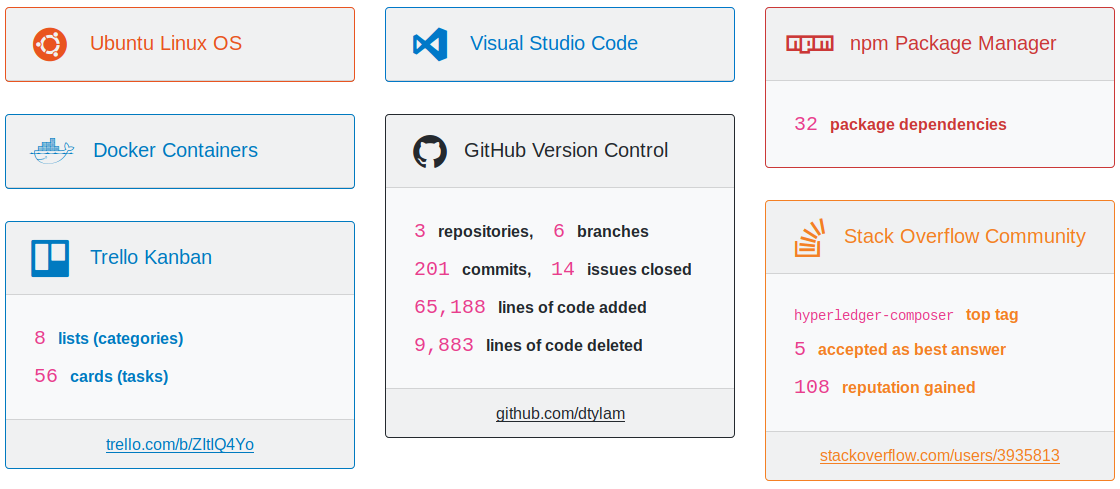
\includegraphics[width=1.0\textwidth]{platform_stats}
	\caption[Development Tools and Usage Statistics]
	{A visual overview of the tools used and their usage statistics if any}
	\label{fig:platform_stats}
\end{figure}

Specific systems and tools were used to build the demonstrator network and client applications (as in Figure \ref{fig:platform_stats}).
These choices and their rationale are detailed below:

\underline{Operating System}: The developer's guide for both Hyperledger Composer and Hyperledger Fabric
recommends using Ubuntu or Mac OS as the host operating system for development.
Ubuntu is selected for being the free and open source option. The development personal computer, which was originally
a Windows machine, was set up to dual boot with the latest Ubuntu release.

\underline{Version Control}: A version control system or software keeps track of source code modifications,
so that developers can compare earlier versions of the code, revert changes, and
minimise disruptions of mistakes \citep{atlassian2018vcs}. It is essential to medium to large scaled projects.

All work done at the implementation stage was tracked with the version control system Git.
Git is a distributed version control system, where repositories can be backed up to a remote server,
such as on the cloud. This is done with GitHub, a git-based version control, code hosting and
project management service that offers free private repositories to verified students \citep{github2018education}.

\underline{Code Editor}: The Hyperledger Composer framework does not require a dedicated integrated
development environment and recommends using a text editor. Visual Studio Code, an open source text editor developed
by Microsoft was chosen as it has a dedicated official syntax checking and beautifying plugin for Hyperledger Composer.

\underline{Community Support}: Hyperledger Composer and Hyperledger Fabric have active communities on Stack Overflow,
a popular online community forums for developers to discuss coding problems. Throughout the duration of the project,
it has been a source of solutions to common problems faced and solved by many other users. Towards the end of the project,
answer contributions were also made.

Several other tools were also used, for example, as previously mentioned in Chapter 3, Trello was used to manage
feature prioritisation for the agile development process. The use of Docker containers and npm package manager
will be explained in due course below.

\section{Architecture and Tech Stack}

\begin{figure}[!ht]
	\centering
	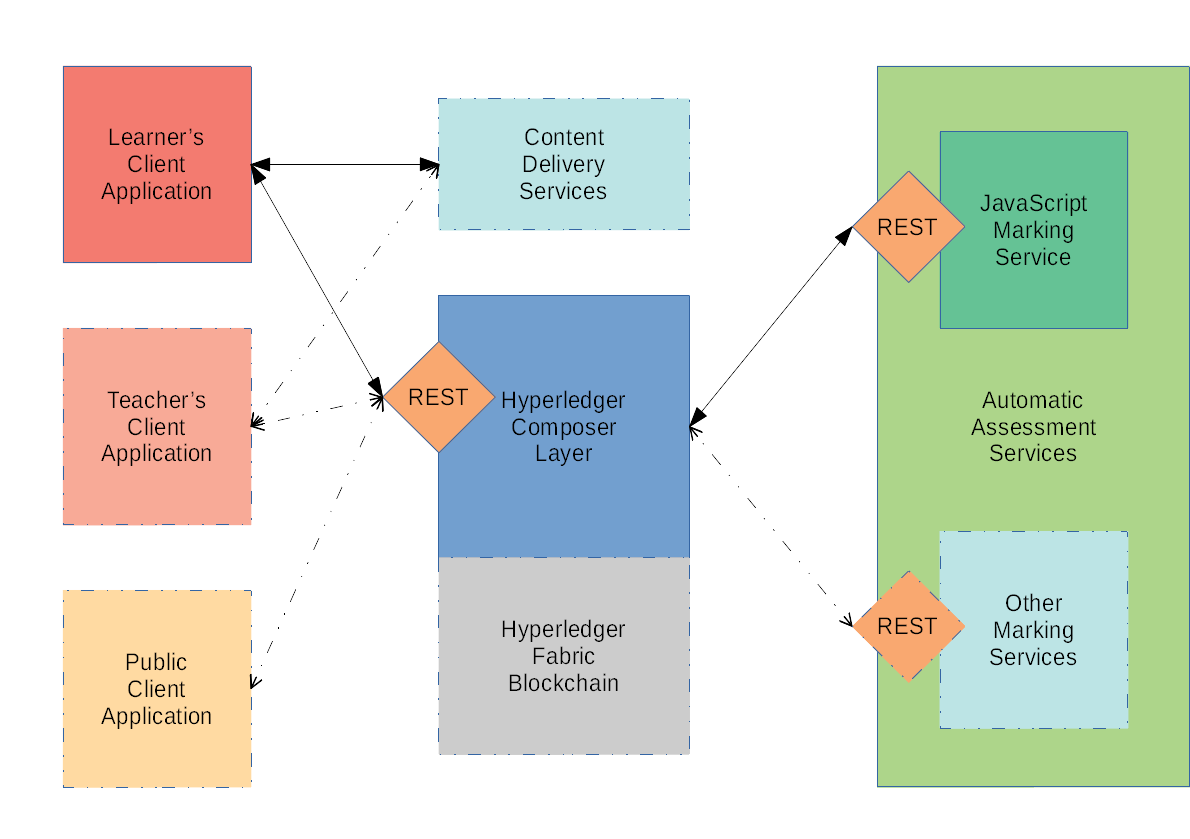
\includegraphics[width=0.9\textwidth]{architecture}
	\caption[Demonstrator Component Architecture]
	{Component architecture overview for the demonstrator system built (dashed lines components were not built)}
	\label{fig:architecture}
\end{figure}

The microservices architecture pattern is used to design the demonstrator system. Microservices is a pattern proposed by
\citet{richardson2018ms} that structures a system as a set of loosely coupled, collaborating services, partitioned so that
each service corresponds to a business capability.

In the demonstrator system (as in Figure \ref{fig:architecture}), this is exemplified by the separation of teacher and student applications,
the separation of content delivery and student records (blockchain), and the separation of different automatic marking services.
They communicate through RESTful web protocols (HTTP and JSON).
This also enables the use of different technologies, separate testing and deployment for each component.

Figure \ref{fig:techstack} shows an alternate overview of the demonstrator system with its technology stack.
These main software packages are described further below.

\begin{figure}[!ht]
	\centering
	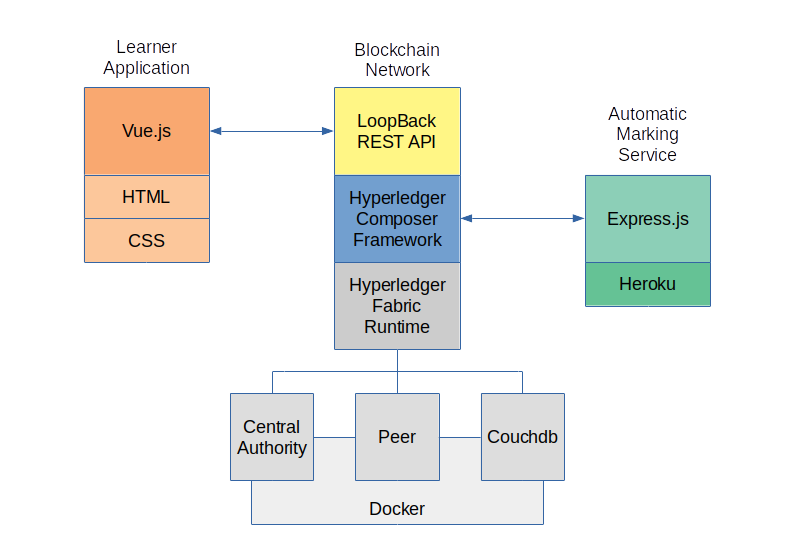
\includegraphics[width=0.85\textwidth]{techstack}
	\caption[Demonstrator Technology Stack]
	{Technology Stack overview for the demonstrator system built}
	\label{fig:techstack}
\end{figure}

\subsection{Client Applications}

The client applications for learners and teachers has to be highly dynamic (non-static) web applications,
with the JavaScript scripting language facilitating most of the user interactions.

Vue.js is a JavaScript-based framework for developing web interfaces. Vue.js was chosen over other
popular frameworks such as React.js and Angular.js because it is focused on the view layer and is much
simpler and faster to learn. The Node.js JavaScript runtime is used to run the Vue.js applications. The npm package manager
is used to install and manage the packages used. See more details such as version numbers in Appendix B.1.

\subsection{Blockchain Network}

Hyperledger Composer deploys to Hyperledger Fabric, which runs on Docker.
Docker is a containerisation platform used to develop distributed systems.
A container is a lightweight, stand-alone package of a piece of software that includes everything
needed to run it from code and tools to system settings.

Docker can emulate multiple servers and run them separately on one development machine.
This provides the peers network needed to host the distributed ledger required for the
Hyperledger Fabric blockchain. A minimum of three docker containers are required to start a
Fabric blockchain: the Central Authority server, a minimum of one peer server, and a Couchdb server,
which is a database that stores the state of the blockchain in a queryable form.

See the full list of pre-requisites and dependencies in in Appendix B.2.

\subsection{Automatic Marking Service}

More automatic marking services were originally planned but due to time constraints only
a simple JavaScript server that checks for file equivalence was implemented.

This was written with Express.js, a minimal Node.js web application framework and hosted
on Heroku, a Node.js capable cloud platform with a free tier. See the full list of pre-requisites and dependencies in in Appendix B.3.

\section{Blockchain Network Development}

Beginning here, progress descriptions and evidences of implementation work will be presented.

\subsection{Command Line Interface}
Using Docker, setup images of Hyperledger Fabric were downloaded, the basic three servers were set up
and a certificate for the central authority administrator was generated. This allows Hyperledger Composer
to later authenticate as the blockchain administrator and import custom network definitions.

The Hyperledger Composer notations from the design phase where packaged into
a business network archive (.bna) file, and deployed to the Hyperledger Fabric blockchain.

Three bash shell scripts were written:
\begin{enumerate}
	\setlength\itemsep{0em}
	\item \textit{start.sh}: this script starts Hyperledger Fabric, generate the minimum number of peers,
	      and connects as the blockchain administrator. It then creates the .bna file with Hyperledger Composer
	      and deploys it to the Fabric blockchain.
	      See Figure \ref{fig:startsh} for a screenshot of the script running.
	      \begin{figure}[!ht]
		      \centering
		      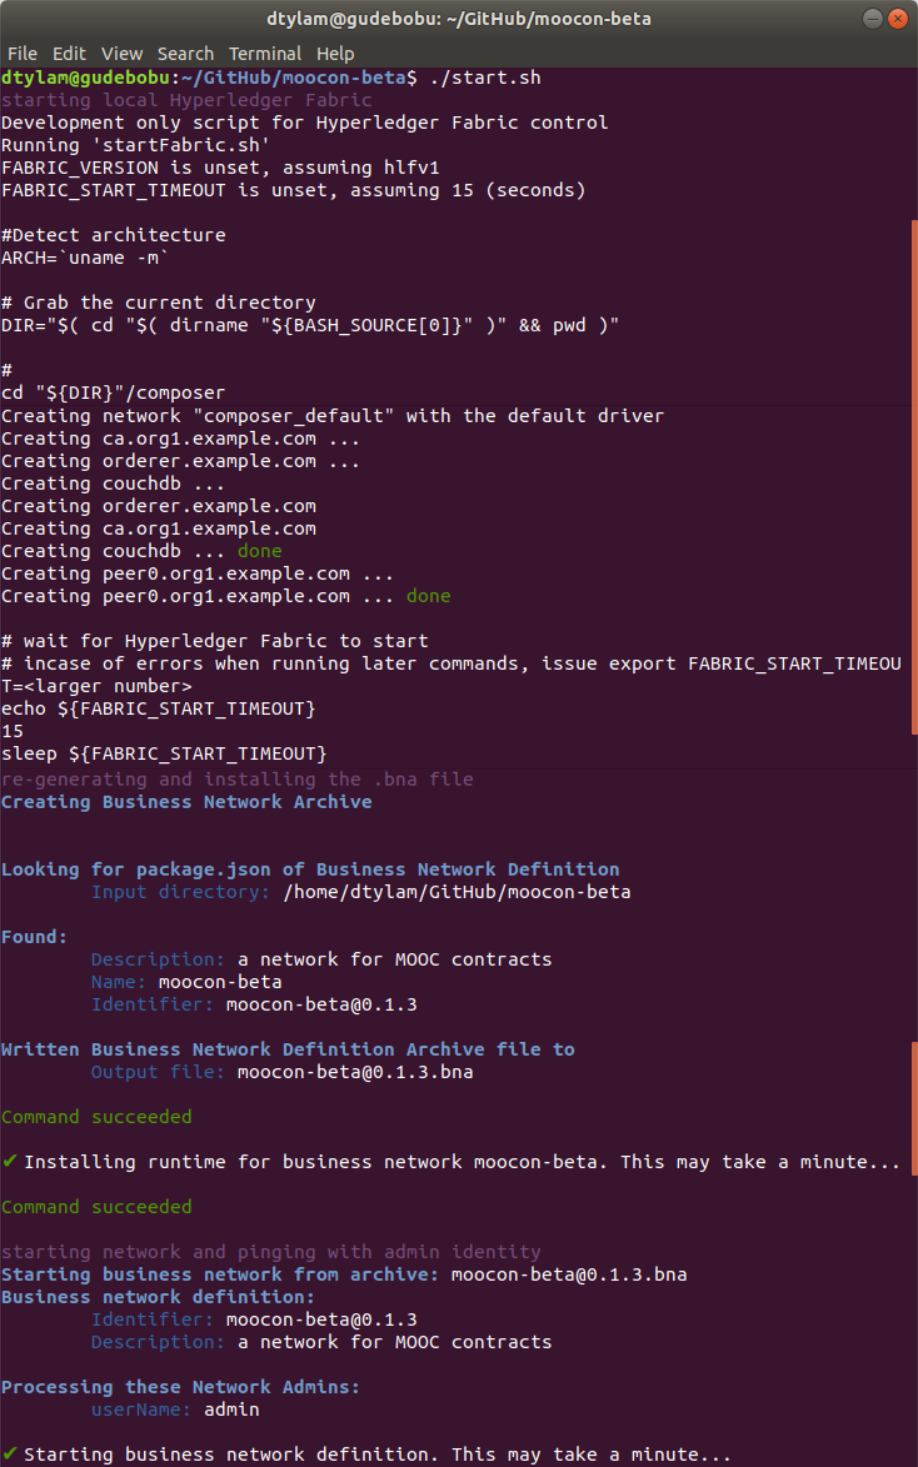
\includegraphics[width=0.85\textwidth]{startsh}
		      \caption[Blockchain Startup Script Screenshot]
		      {Screenshot of the start.sh script in action in a command line interface}
		      \label{fig:startsh}
	      \end{figure}
	\item \textit{load\_participant.sh}: this script connects as the blockchain administrator and creates
	      three \textit{Learner}, four \textit{Teacher} and two \textit{Reader} participants on the blockchain.
	      A .card file is created for each participant, which contains the certificate they need to
	      connect to the blockchain as themselves. In the final stages of development, this script is called by
	      the previous \textit{start.sh} to simplify the starting and loading process.
	      See Figure \ref{fig:load_participantsh} for a screenshot of the script running.
	      \begin{figure}[!ht]
		      \centering
		      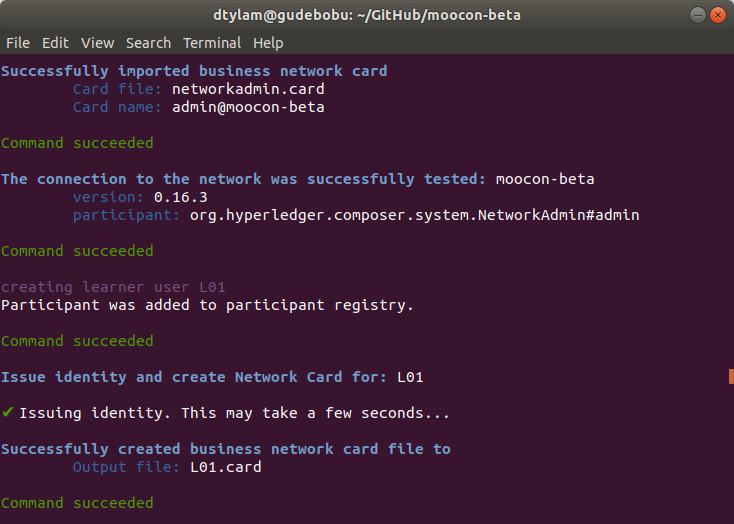
\includegraphics[width=0.85\textwidth]{load_participantsh}
		      \caption[Participant Loading Script Screenshot]
		      {Screenshot of the load\_participant.sh script in action in a command line interface}
		      \label{fig:load_participantsh}
	      \end{figure}
	\item \textit{destroy.sh}: at the end of every development session the blockchain is completely
	      erased and removed. This is because unwanted data entries or transactions may have occurred, and
	      the blockchain schema can only be changed with a hard fork/ restart.
	      See Figure \ref{fig:destroysh} for a screenshot of the script running.
	      \begin{figure}[!ht]
		      \centering
		      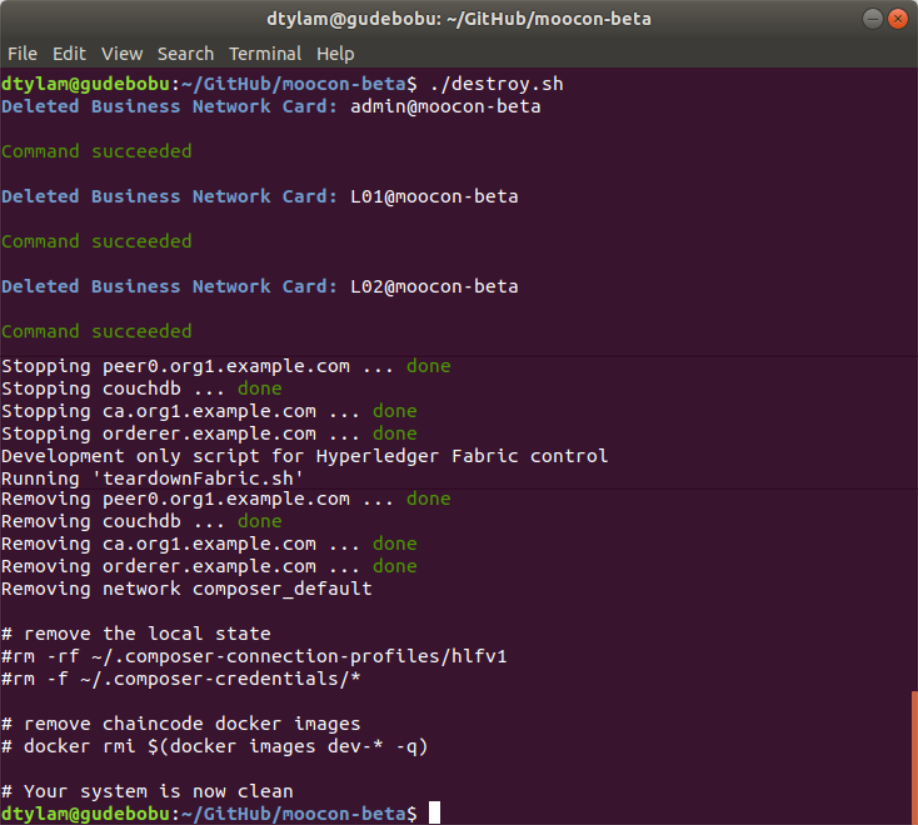
\includegraphics[width=0.85\textwidth]{destroysh}
		      \caption[Blockchain Teardown Script Screenshot]
		      {Screenshot of the destroy.sh script in action in a command line interface}
		      \label{fig:destroysh}
	      \end{figure}
\end{enumerate}

The GitHub source code repository used for the blockchain schema and command line scripting
is hosted at \href{https://github.com/dtylam/moocon-beta}{\underline{github.com/dtylam/moocon-beta}}.
Three branches (significant iterations) were created for this component, below in chronological order:
\begin{enumerate}
	\setlength\itemsep{0em}
	\item \textit{moocon-alpha} branch: this is an archived repository of design work done with version 0.15.x of
	      Hyperledger Composer, the project upgraded to version 0.16 in December, which contained breaking changes.
	      The 0.16 upgrade was recommended by the Hyperledger developers because it is a long term support
	      release that is feature complete and stable, and adds the useful .card file authentication protocol.
	\item \textit{master} branch: this is the original working branch on Hyperledger Composer 0.16, a bulk of
	      design and development work was done, and changes to the schema and transactions were made based on
	      literature review and background research.
	\item \textit{bcu} branch: this is the final, demonstration ready branch named after the proposed marketplace
	      "Blockchain University". Changes were made to satisfy new requirements obtained through primary data (interviews in Chapter 4).
\end{enumerate}

\subsection{Application Program Interface}

A readily available script connects the deployed blockchain to Loopback, an open source Node.js RESTful
Application Program Interface (API) framework. The command used is:

\begin{verbatim}
	composer-rest-server --card admin@moocon-beta --namespaces always 
	--websockets true --port 3000 --authentication true --multiuser true
\end{verbatim}

This hosts a production-ready API at \texttt{localhost:3000}, connected to the
server of the central authority administrator.
Figure \ref{fig:Loopback_explorer} shows the API explorer view generated by Loopback at \texttt{localhost:3000/explorer}.

\begin{figure}[!ht]
	\centering
	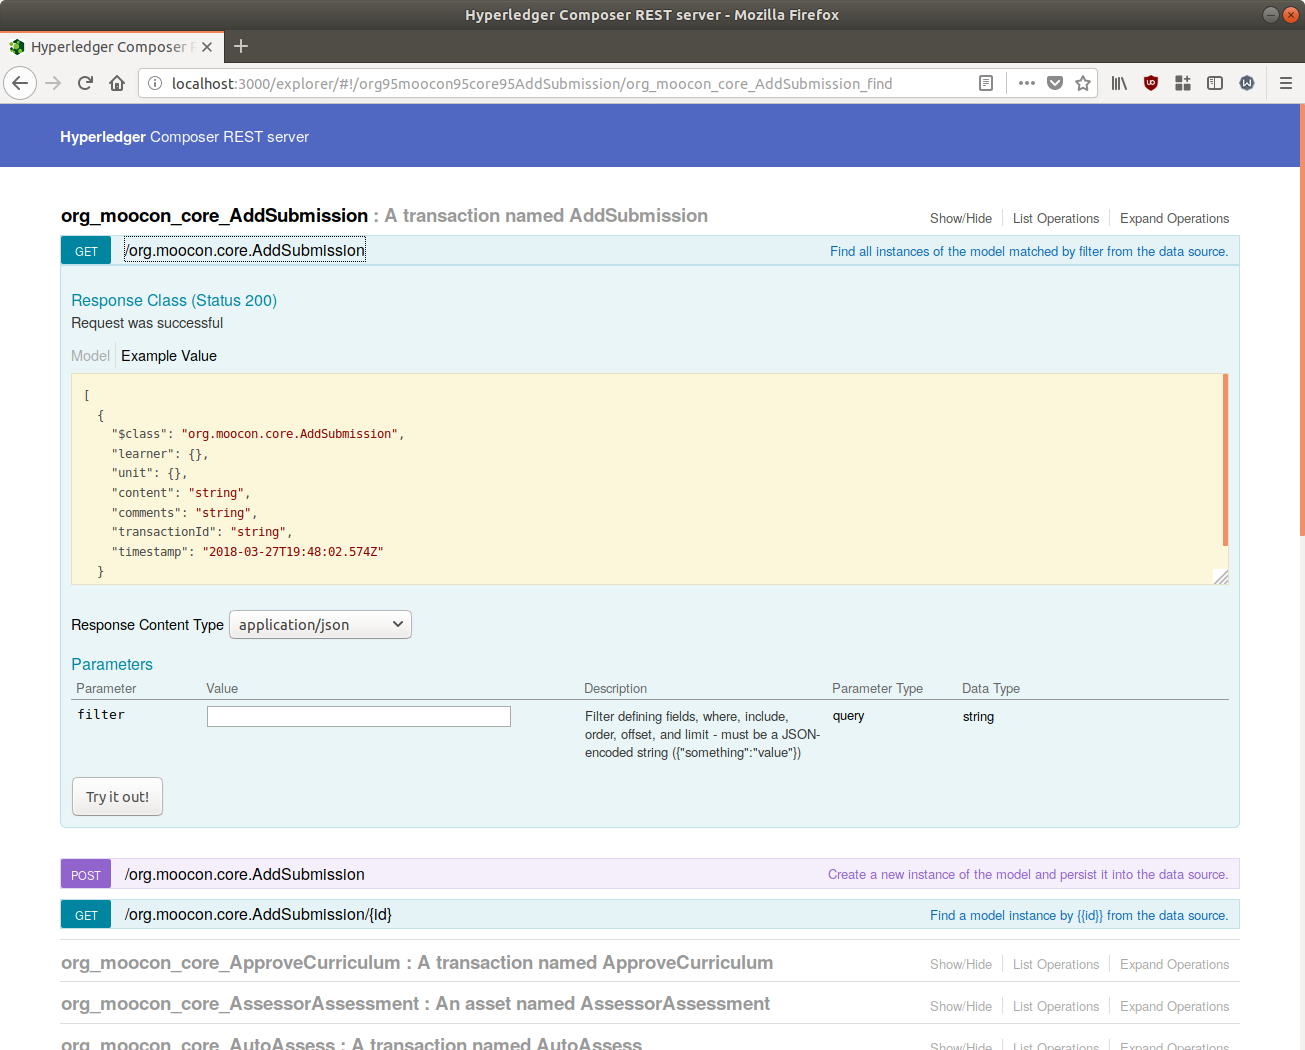
\includegraphics[width=1.0\textwidth]{Loopback_explorer}
	\caption[Hyperledger Composer Loopback REST API Screenshot]
	{Screenshot of the auto-generated Loopback Explorer for the blockchain according to Hyperledger Composer definitions}
	\label{fig:Loopback_explorer}
\end{figure}

Limitations exist for how multiple participants can use this same API. The API is authenticated as
one peer at one time. It uses a construct called \texttt{wallet} to store .card files and
switches between them to create a "multiuser" API. So to switch between users in the
client applications, a request must be made to \texttt{localhost:3000/wallet/\{cardFileName\}/setDefault}.
This limitation is accepted for the demonstrator system, as it does not impact core requirements.

\section{Automatic Marking Service Development}

The first iteration of the Blockchain Network has no automatic marking Smart Contract features.
This is due to a limitation found during development of the original design. The original design
of the Automatic Assessment Smart Contract would have the Smart Contract run a custom block of chaincode
created by a Teacher for each assessment (See left hand side of Figure \ref{fig:automarkinglim}).

However, the Hyperledger Composer framework does not allow chaincode to run code foreign to its main packages and vanilla JavaScript.
This is due to the transpilation and deployment of Hyperledger Composer chaincode to the Hyperledger Fabric blockchain,
a process which ordinary developers have no convenient controls over. It will not be able to accept new snippets of code,
created and uploaded to the blockchain by Teacher participants.

\begin{figure}[!ht]
	\centering
	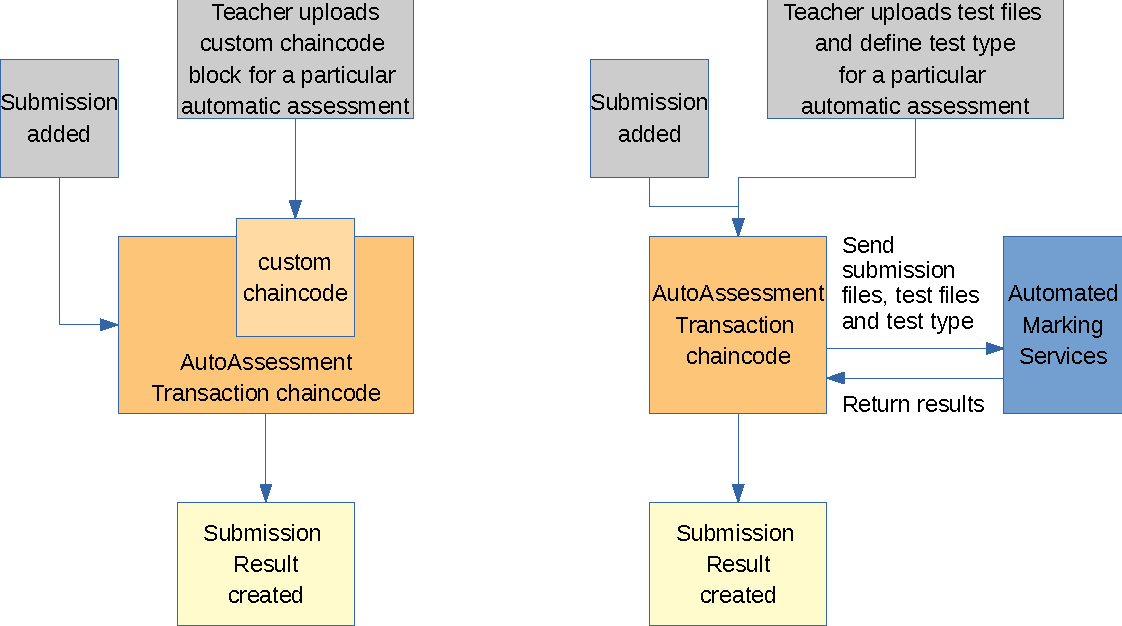
\includegraphics[width=0.9\textwidth]{automarkinglim}
	\caption[AutoAssessment Smart Contract Design Change]
	{Flowchart of original design (left) and the technically informed design (right) of how the Automatic Assessment Smart Contract should run}
	\label{fig:automarkinglim}
\end{figure}

Understanding this limitation and after studying documentations further, a technically informed design was created
(See right hand side of Figure \ref{fig:automarkinglim}). he Hyperledger Composer framework allows chaincode
to communicate with external APIs through a built-in method \texttt{post(url,data)} where \texttt{url} is
the endpoint address of the desired API and \texttt{data} is a blockchain asset or concept serialised into JSON format.

This limitation and subsequent redesign has actually inspired the microservices architectural approach covered in the previous section 6.1.

To use the \texttt{post(url,data)} functionality effectively, an extra asset \textit{AutoAssessRequest} was added to the blockchain schema.
\textit{AutoAssessRequest} would contain the submission content file, the test file on the blockchain for this assessment, the test type of
this assessment (eg. software testing, AI testing, etc), and an API response field. This packages all the information the external
Automated Marking Services will need, and keep the request and response records permanently on the blockchain.

To build an example automated marking service, a string equivalence test was created on a simple Express.js application server.
Here is the simple code snippet used:
\begin{verbatim}
if (req.body.testFile === req.body.content) {
    res.json(true); // if the test file is equal to the submission file
} else { res.json(false); } 
\end{verbatim}

Even though this is just a simple equivalence test, it proves the blockchain's ability to conduct automated assessments, 
and more sophisticated assessment APIs could be called or routed to.

It is essential that this testing service is available on the world-wide web, because the peers are contained in Docker
containers where the normal workstation \texttt{localhost} address is not easily reachable. Therefore, the heroku Node.js 
hosting service is used and this example automated marking service is available at 
\href{https://moocon-js-marking.herokuapp.com/}{\underline{moocon-js-marking.herokuapp.com/}}.

The source code of this component is also tracked and hosted at 
\href{https://github.com/dtylam/moocon-js-marking}{\underline{github.com/dtylam/moocon-js-marking}}.

\section{Client Applications Development}

Before developing the client applications, some example data was created and imported into the network. 
This was nine courses modules, their module units and assessments. These data were created by loosely following 
the syllabuses of courses from Massive Open Online Courses.

A video demonstration showcasing the user journeys across both applications was created and 
available on \href{https://youtu.be/FUMBn6wPG5M}{\underline{youtube.com/FUMBn6wPG5M}}.

An open source styling and component library, \href{https://vuematerial.io/}{Vue-material}, was used to 
create Material Design compliant user interfaces. Notes on the development process are further detailed below.

\subsection{Learner Application}

The source code of this application is tracked and hosted at 
\href{https://github.com/dtylam/moocon-learner-client}{\underline{github.com/dtylam/moocon-learner-client}}.
Two branches (significant iterations) were created for this component, below in chronological order:
\begin{enumerate}
	\setlength\itemsep{0em}
	\item \textit{master} branch: this is the first iteration made based on literature review and background research.
	\item \textit{bcu} branch: this is the final, demonstration ready branch. 
	Changes were made to satisfy new requirements obtained through primary data (interviews in Chapter 4).
\end{enumerate}

The switch from traditional static webpage development to component-driven development was a steep learning curve.
Traditional web development focuses on the separation of concerns by file types, where markup (HTML), 
styling (CSS) and scripting (JavaScript) are in different files and folders.

JavaScript-based web applications, on the other hand, encourage organisation according to functional components. 
In Vue.js for example, components (.vue) files are used to write HTML, CSS and JavaScript in one file \citep{vue2017components}, 
which creates a component in the web application. It is afterwards packaged to be production-ready with build tools.

For example, the entire web application only uses one main \texttt{index.html} page. Each main menu button 
such as "Ongoing Courses" swaps out the previous page component for another. Components can also be nested, 
the YouTube embedding view is its own component, for example.

Below are some annotated screenshots of the application (Figures to ).

\begin{figure}[!ht]
	\centering
	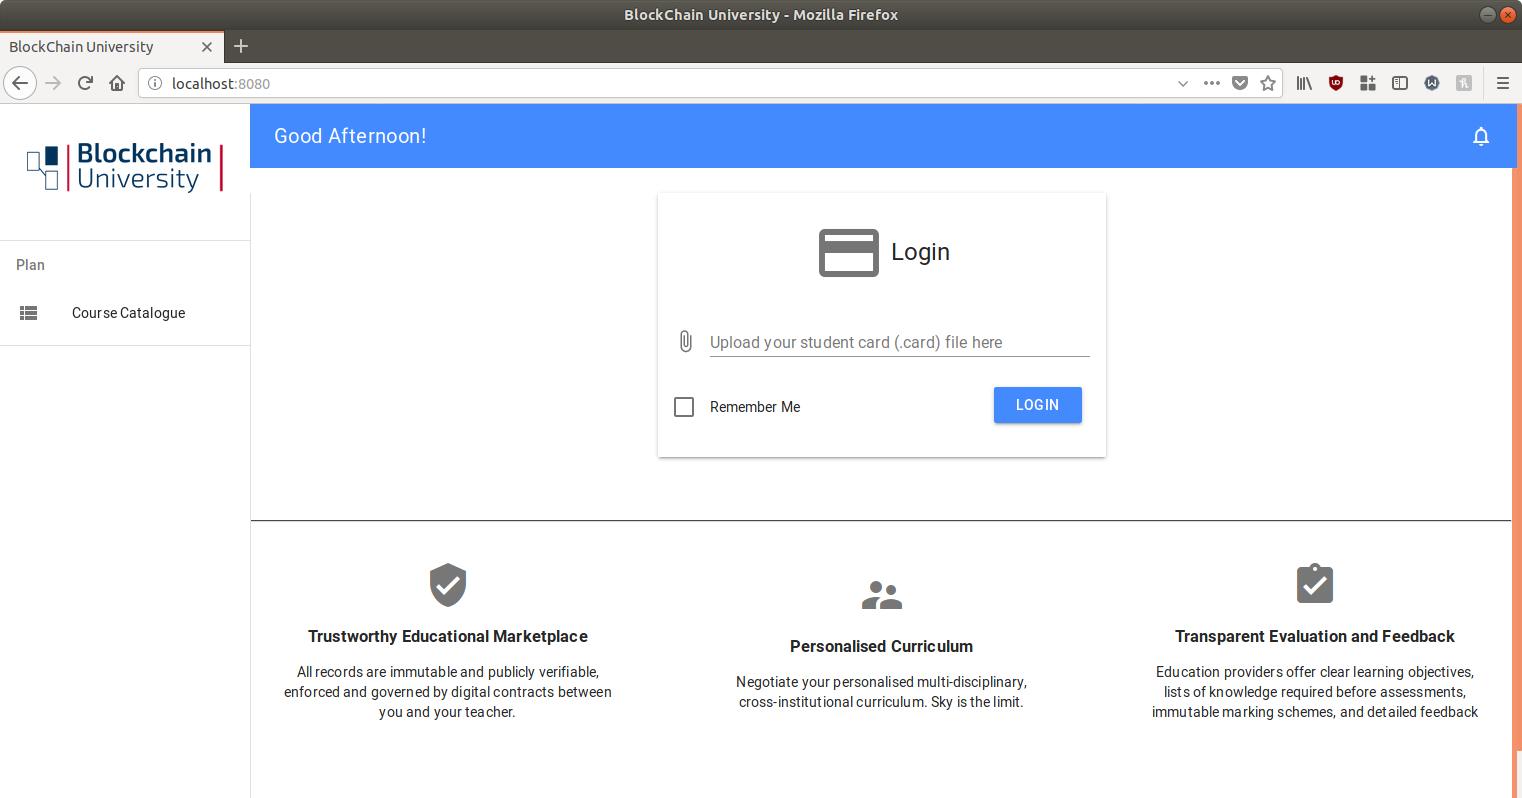
\includegraphics[width=1.0\textwidth]{Learner_login}
	\caption[Learner Application Login Page]
	{Flowchart of original design (left) and the technically informed design (right) of how the Automatic Assessment Smart Contract should run}
	\label{fig:Learner_login}
\end{figure}

\begin{figure}[!ht]
	\centering
	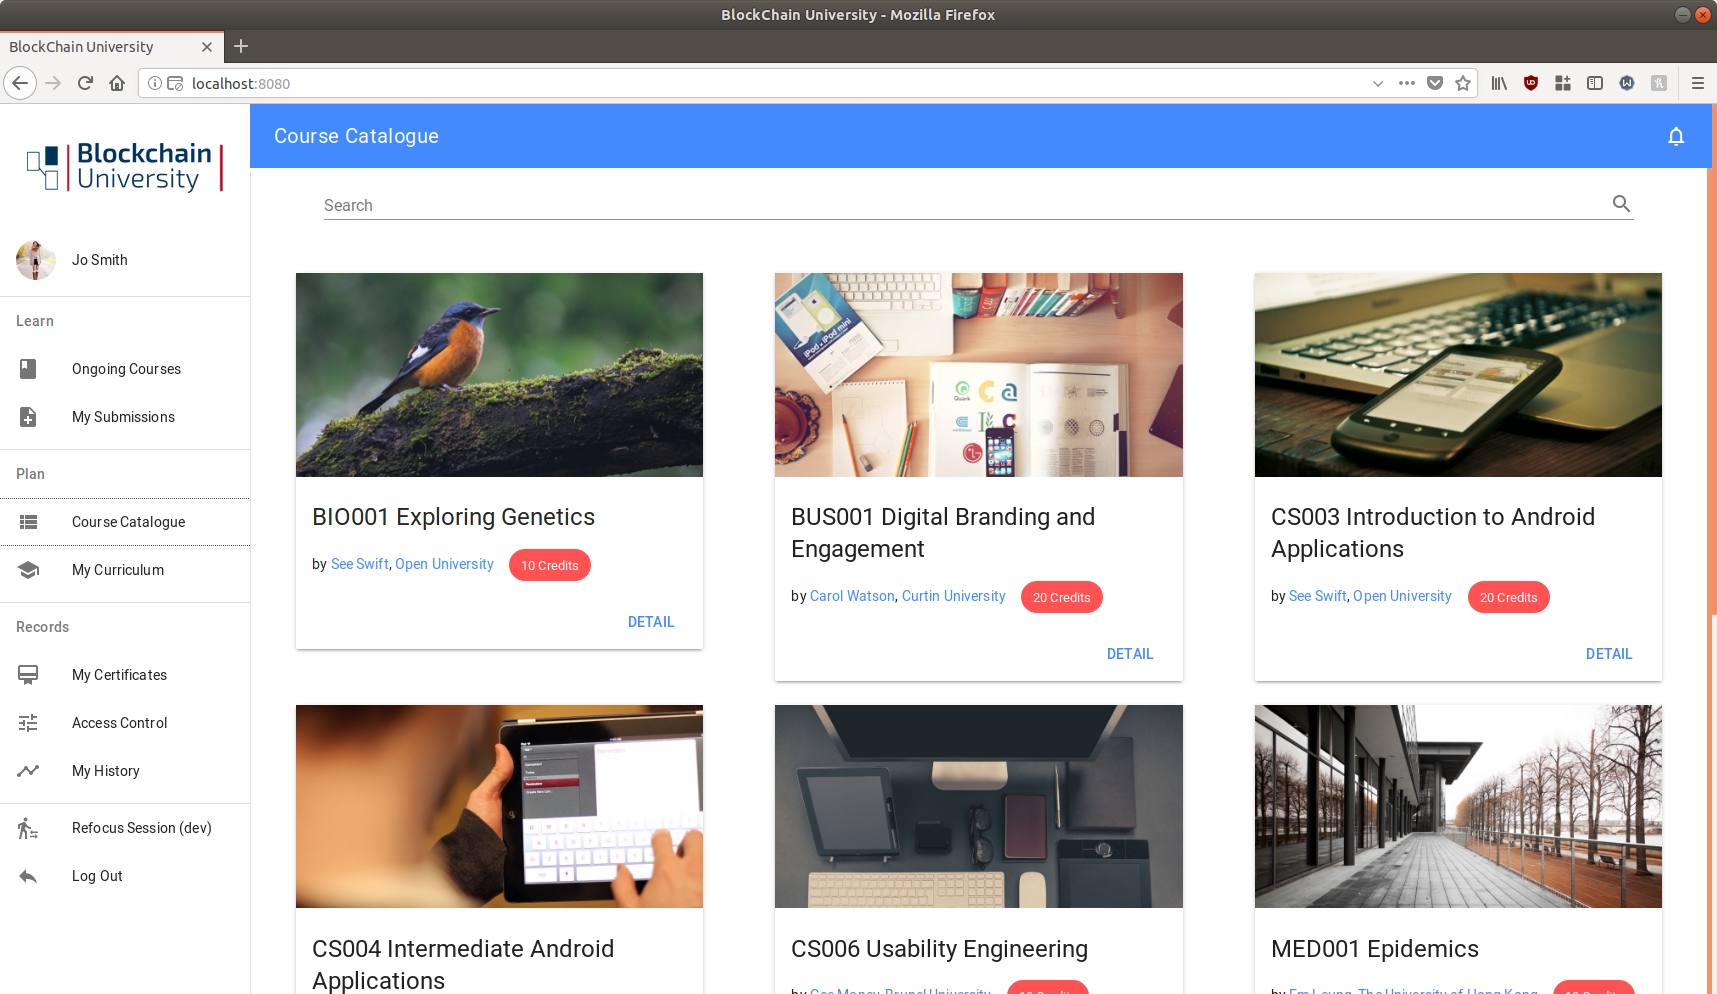
\includegraphics[width=1.0\textwidth]{Learner_allcourses}
	\caption[Learner Application Course Catalogue Page]
	{Flowchart of original design (left) and the technically informed design (right) of how the Automatic Assessment Smart Contract should run}
	\label{fig:Learner_allcourses}
\end{figure}

\begin{figure}[!ht]
	\centering
	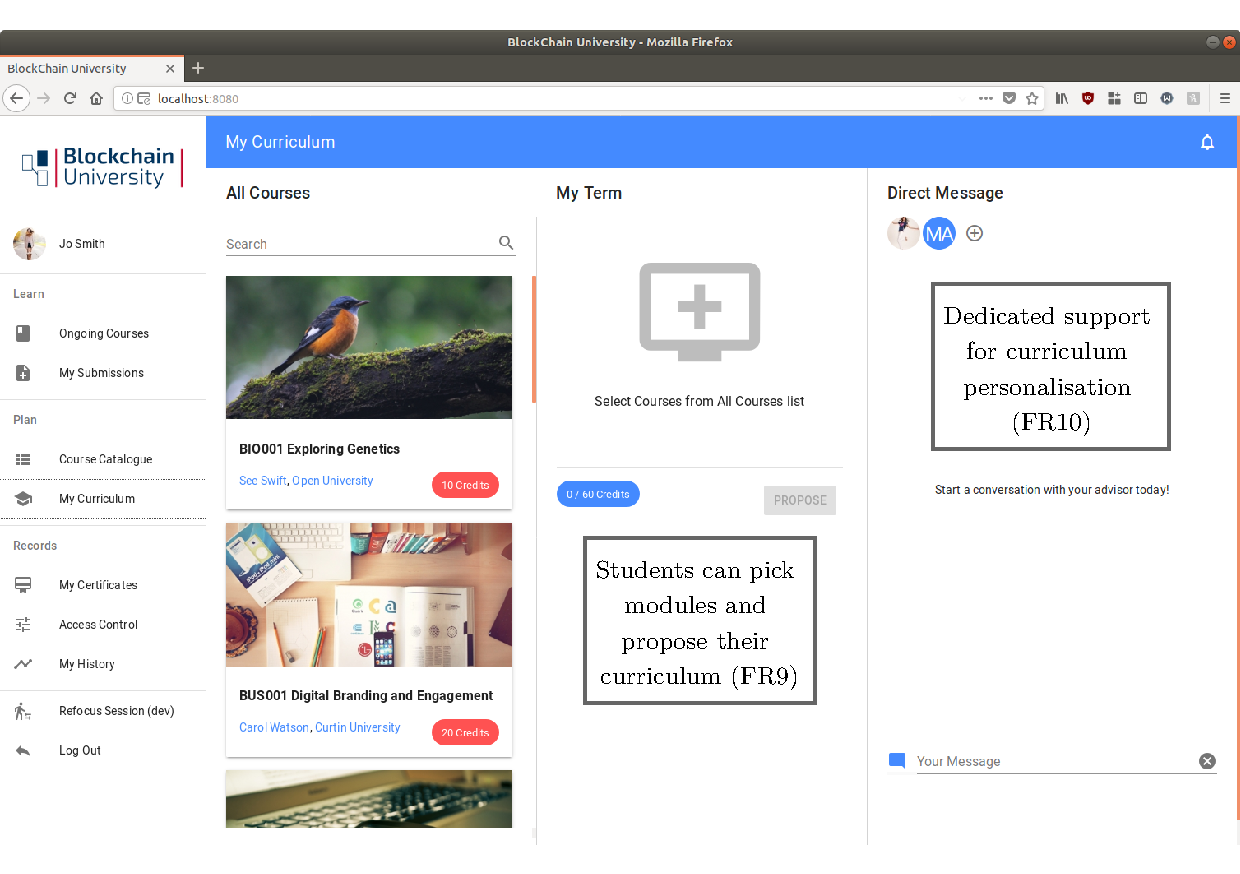
\includegraphics[width=1.0\textwidth]{Learner_customiser}
	\caption[Learner Application My Curriculum Page]
	{Flowchart of original design (left) and the technically informed design (right) of how the Automatic Assessment Smart Contract should run}
	\label{fig:Learner_customiser}
\end{figure}

\begin{figure}[!ht]
	\centering
	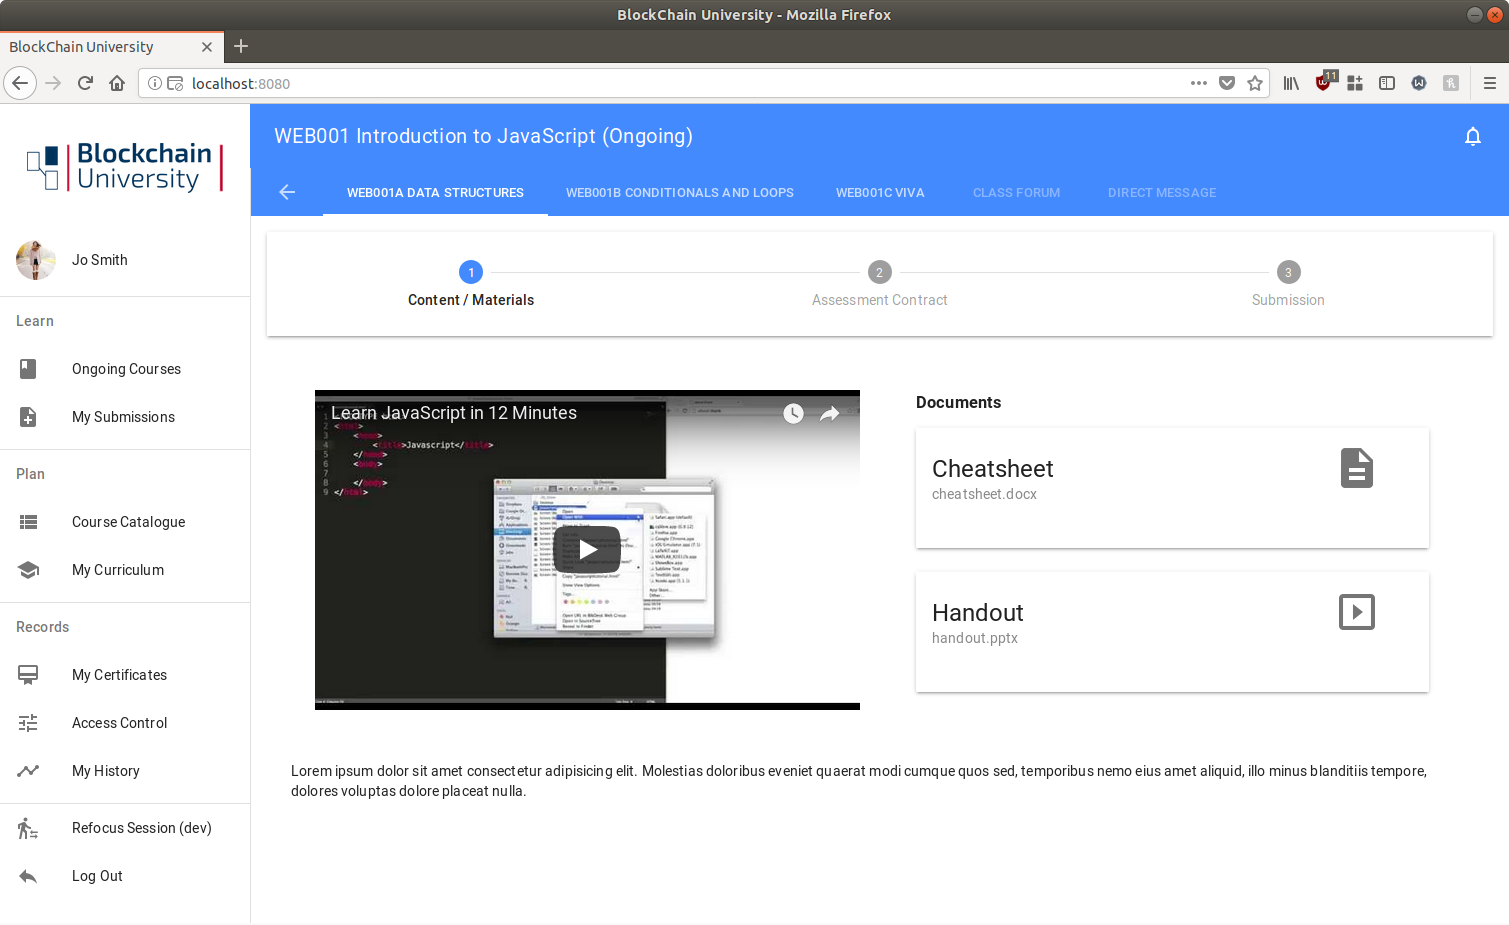
\includegraphics[width=1.0\textwidth]{Learner_ongoing1}
	\caption[Learner Application Example Ongoing Module Page]
	{Flowchart of original design (left) and the technically informed design (right) of how the Automatic Assessment Smart Contract should run}
	\label{fig:Learner_ongoing1}
\end{figure}

\begin{figure}[!ht]
	\centering
	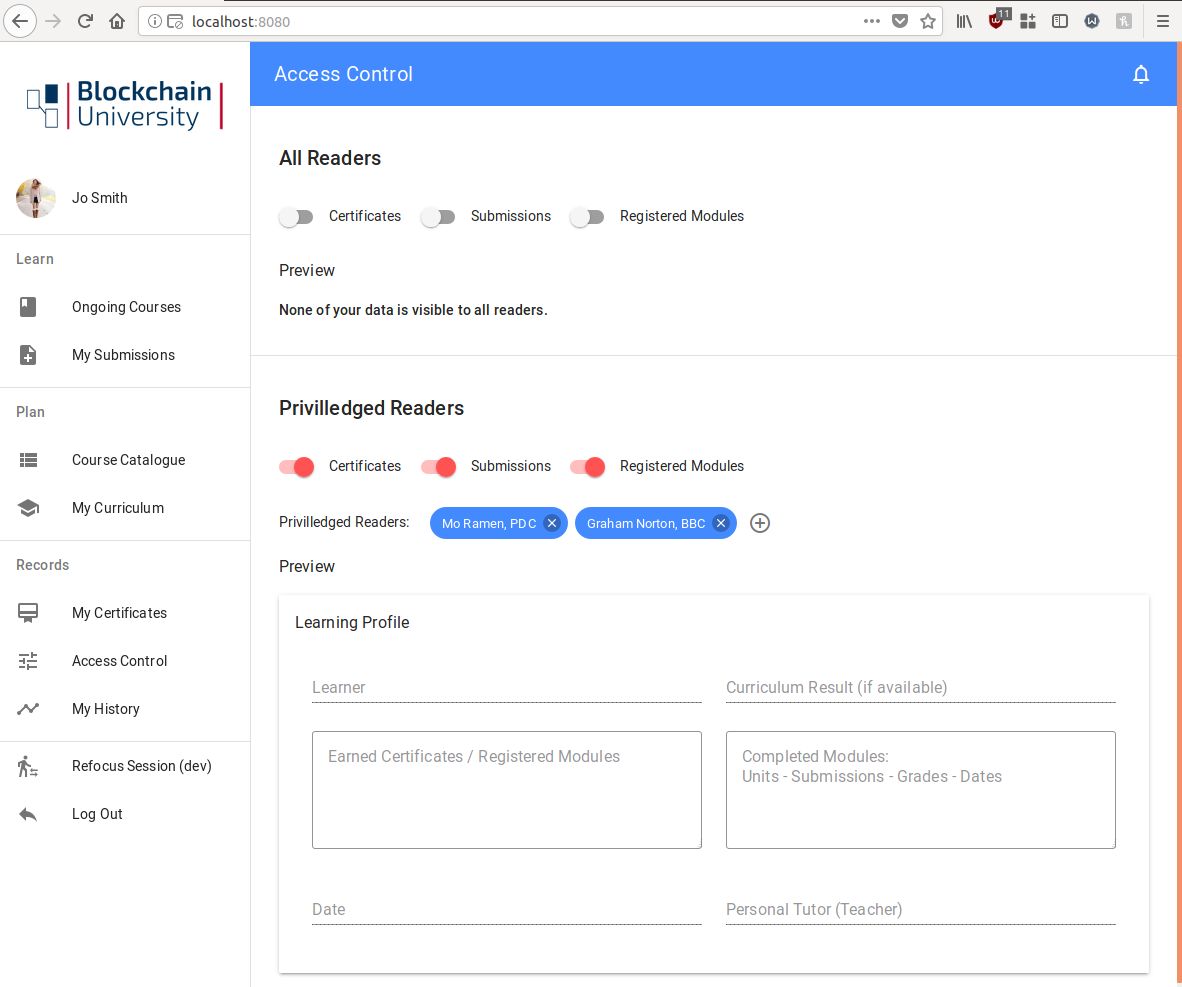
\includegraphics[width=1.0\textwidth]{Learner_AC}
	\caption[Learner Application Access Control Page]
	{Flowchart of original design (left) and the technically informed design (right) of how the Automatic Assessment Smart Contract should run}
	\label{fig:Learner_AC}
\end{figure}

\subsection{Teacher Application}

The Teacher application was created as a fork of the Learner application. 
The source code of this application is tracked and hosted at 
\href{https://github.com/dtylam/moocon-teacher-client}{\underline{github.com/dtylam/moocon-teacher-client}}.
Only one iteration was completed by the end of the project, as this application was built after requirements gathering interviews.

\begin{figure}[!ht]
	\centering
	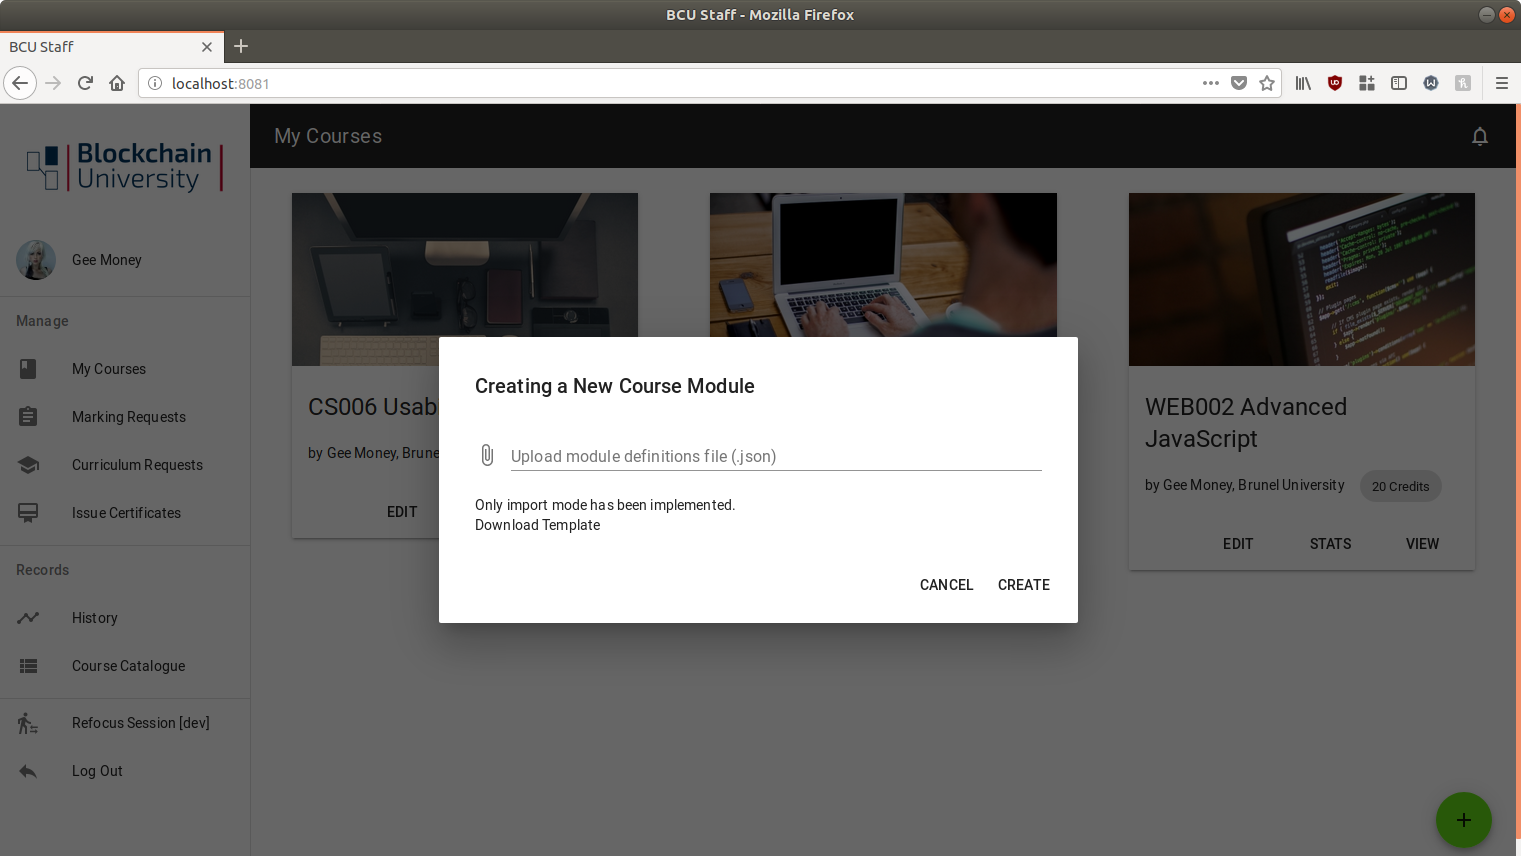
\includegraphics[width=1.0\textwidth]{Teacher_createcourse}
	\caption[Teacher Application My Courses Page]
	{Flowchart of original design (left) and the technically informed design (right) of how the Automatic Assessment Smart Contract should run}
	\label{fig:Teacher_createcourse}
\end{figure}

\begin{figure}[!ht]
	\centering
	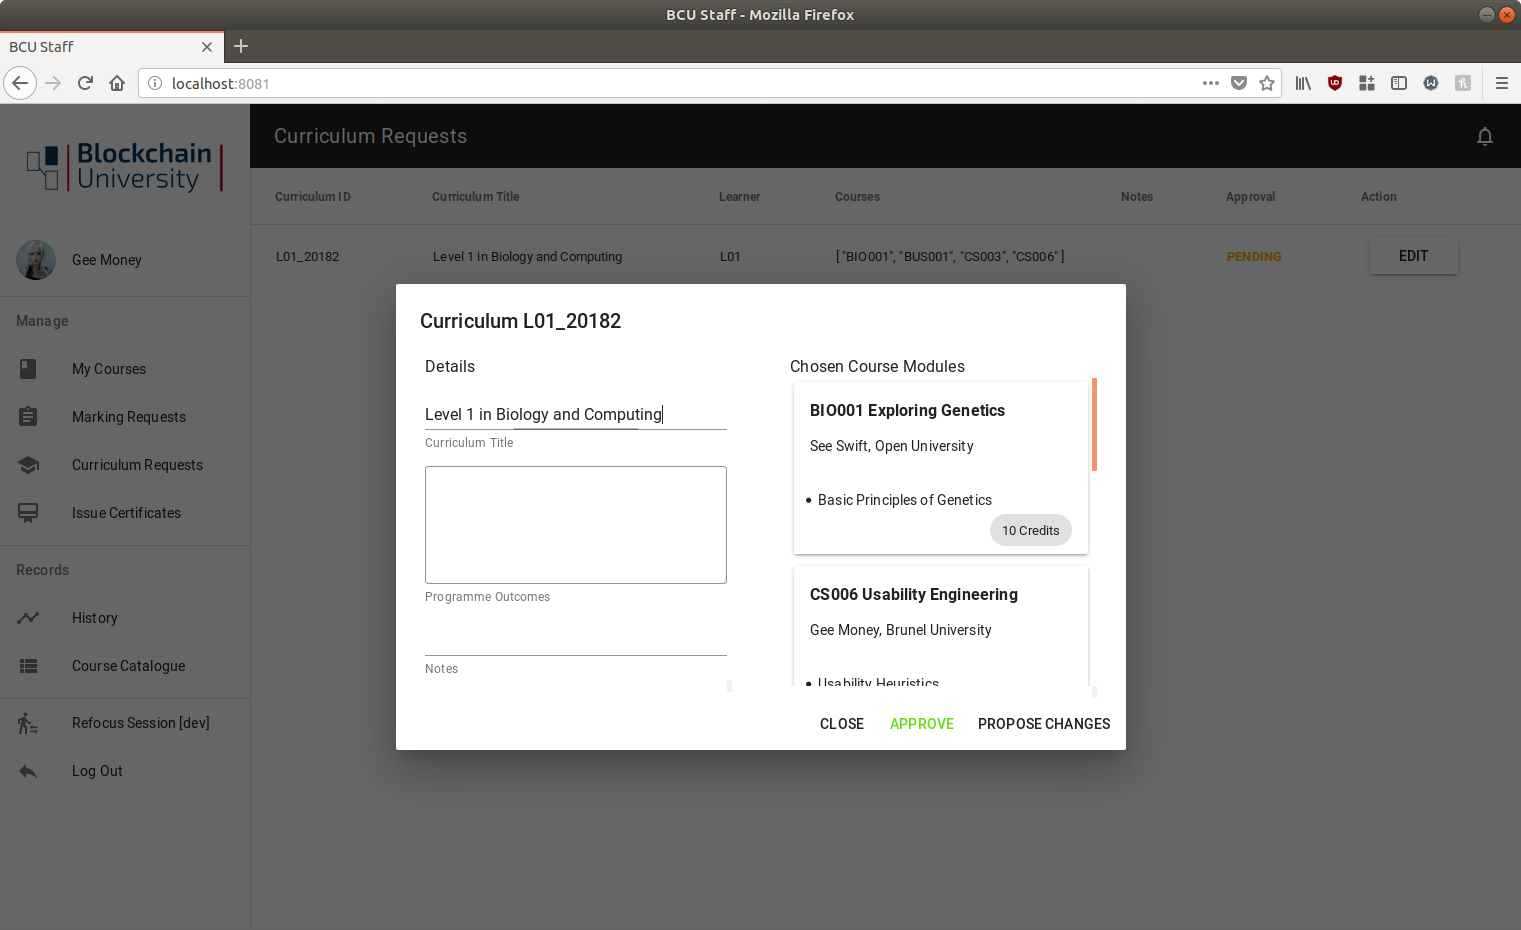
\includegraphics[width=1.0\textwidth]{Teacher_approvecurr}
	\caption[Teacher Application Curriculum Requests Page]
	{Flowchart of original design (left) and the technically informed design (right) of how the Automatic Assessment Smart Contract should run}
	\label{fig:Teacher_approvecurr}
\end{figure}

\begin{figure}[!ht]
	\centering
	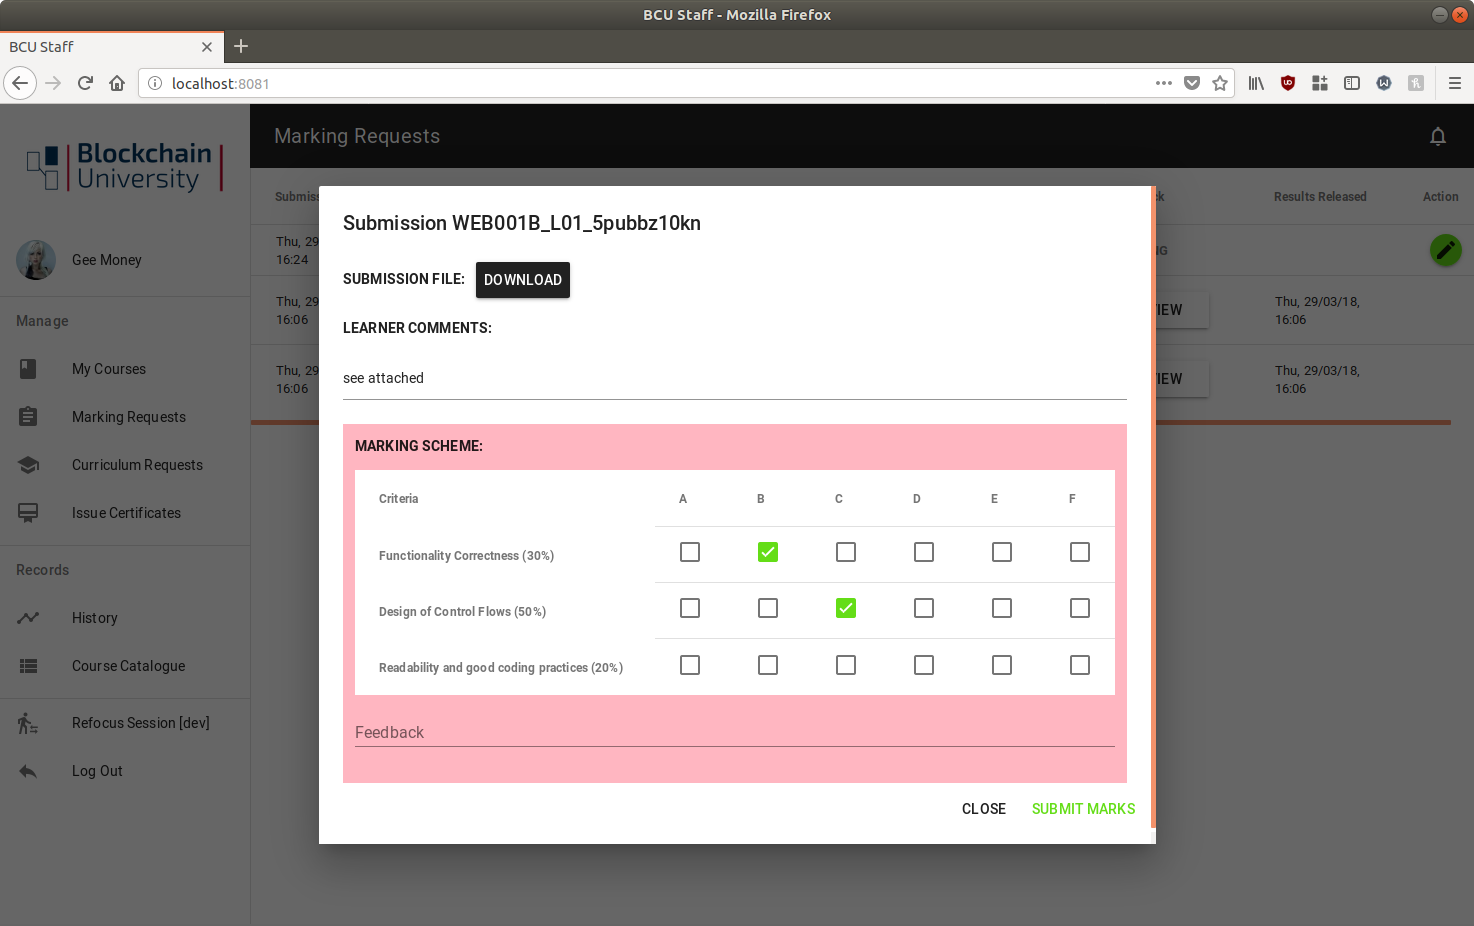
\includegraphics[width=1.0\textwidth]{Teacher_marking}
	\caption[Teacher Application Marking Requests Page]
	{Flowchart of original design (left) and the technically informed design (right) of how the Automatic Assessment Smart Contract should run}
	\label{fig:Teacher_marking}
\end{figure}

\section{Test Driven Development}

Support for unit testing is built-in for Hyperledger Composer with popular JavaScript testing frameworks Mocha and Chai.
Several unit tests were written to test the blockchain network schema and transactions. [TODO expand]

Postman, a popular API testing platform, is used to run whitebox tests against the API 
before and during the development of the client applications. [TODO expand]

\section{Limitations and Issues}

Blockchain Events were being broadcasted network-wide without access control filters. 
Some Events are only targeted at a particular individual but all of the peers will receive it.

For example, only the proposing \textit{Learner} and his/ her personal tutor \textit{Teacher} should 
be receiving the notification that a curriculum has been proposed. Currently, all peers across the 
blockchain receives this notification, but they are blocked at the client application level.

This is a limitation of Hyperledger Composer, which does not provide ways to limit the scope of an \textit{Event}.
It would cause privacy issues for a real-world system, as any actor on the blockchain could potentially 
listen to these \textit{Events} and attempt to create a partial view of user histories.
